\section{3D Reconstruction of the Test Objects}

The calibrated unwrapped phase maps from the previous chapters were viewed in 3D. Their mesh profiles after applying the postprocessing techniques are shown below. 

We can see the differences upon application of each image processing technique for the styrofoam with engravings in Figure \ref{fig:3DV}. 
%The most dominant change for the FFT-filtering part is the styrofoam with engravings. This can be attributed to the flatness of its surface (as compared to the other test objects). 
Notice the transition of its mesh in yz-axis mode from a tilted object to flat but noisy and finally, flat with reduced noise.

\begin{figure}[p]
	\centering
	\subfigure[]{
		{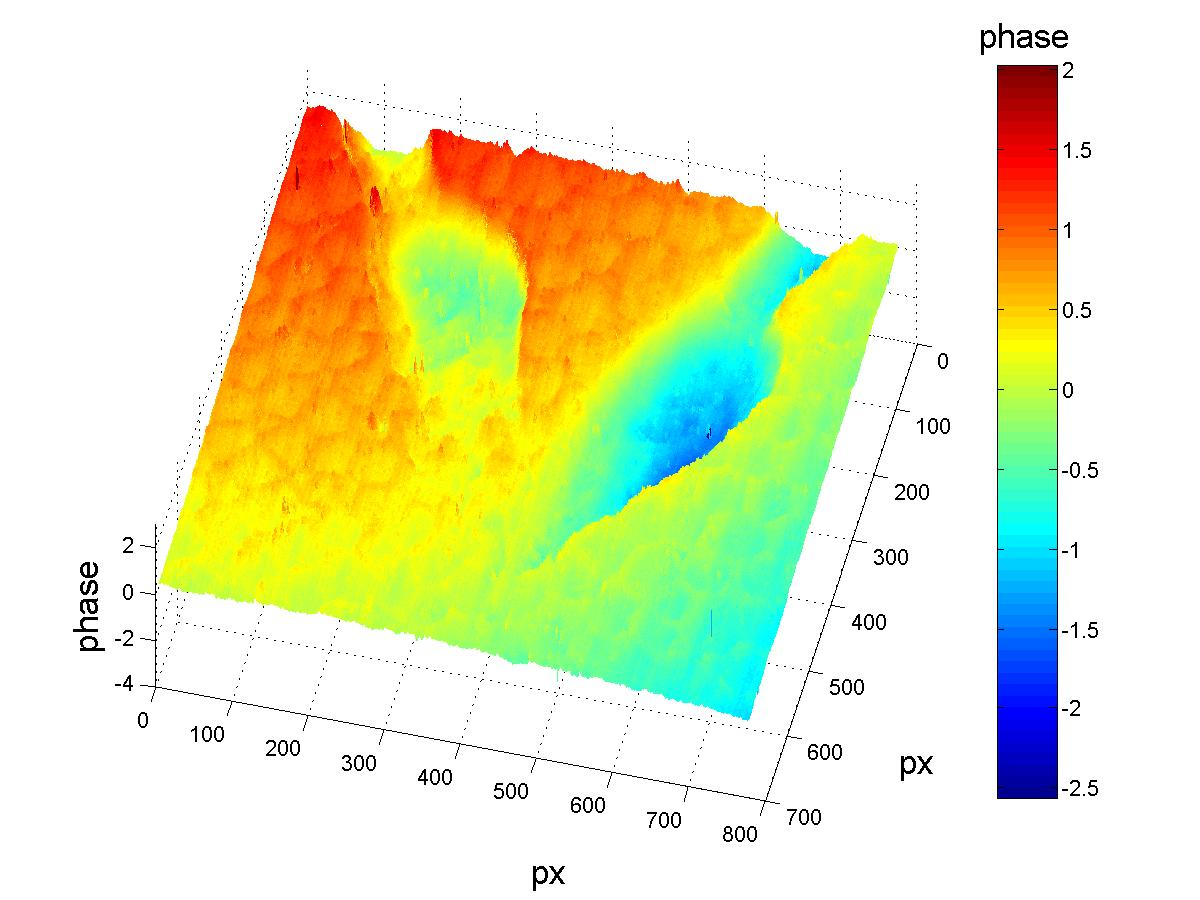
\includegraphics[width=0.5\textwidth]{figures/3Dv.jpg}}
		{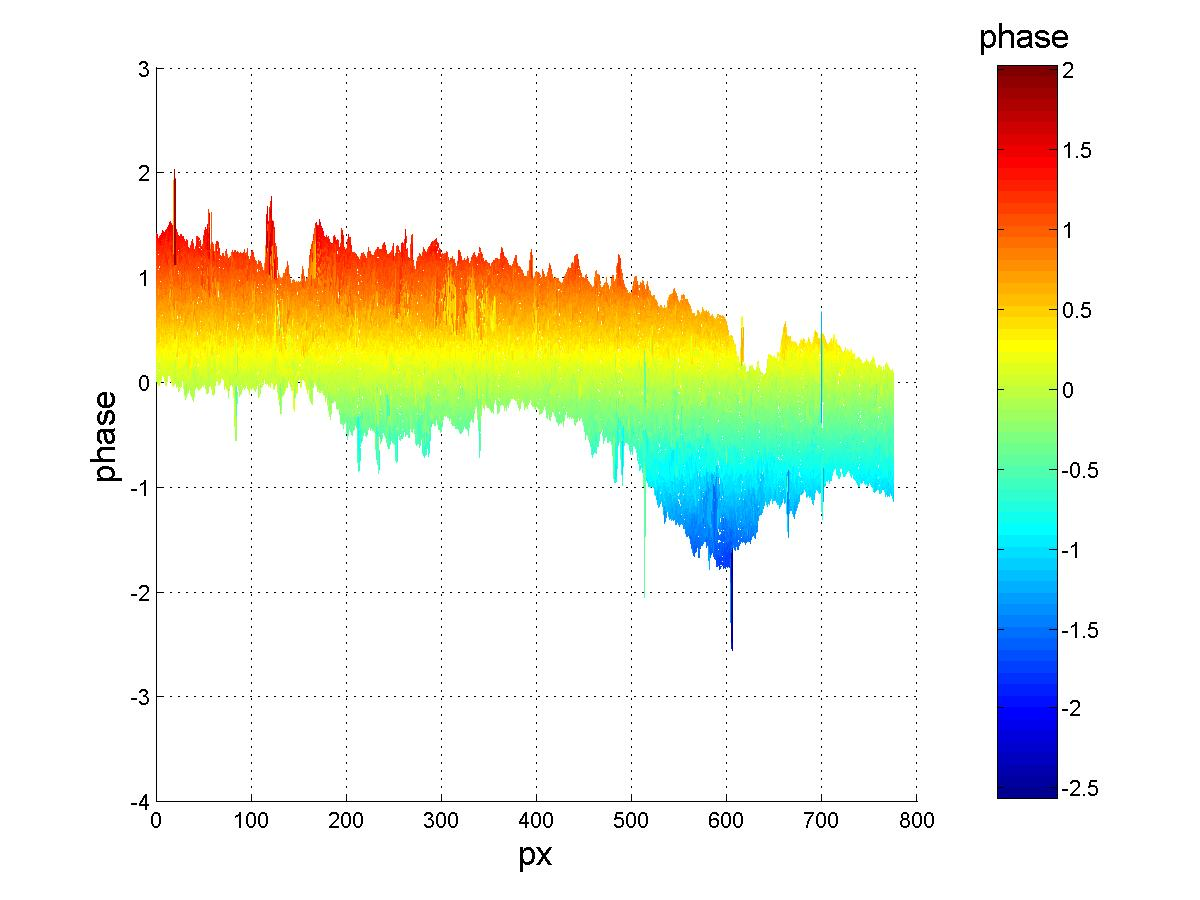
\includegraphics[width=0.5\textwidth]{figures/3Dv_yz.jpg}}}
	\subfigure[]{
		{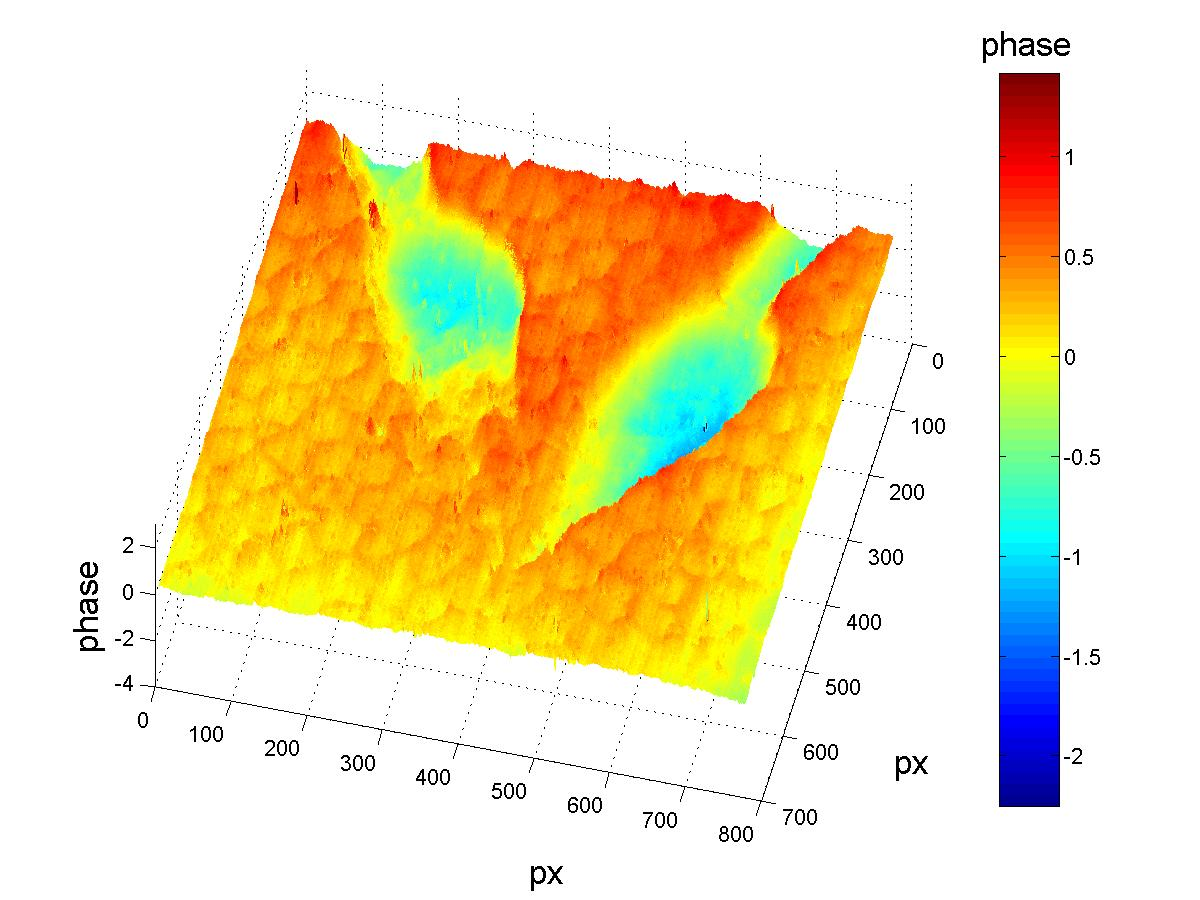
\includegraphics[width=0.5\textwidth]{figures/3DvBS.jpg}}
		{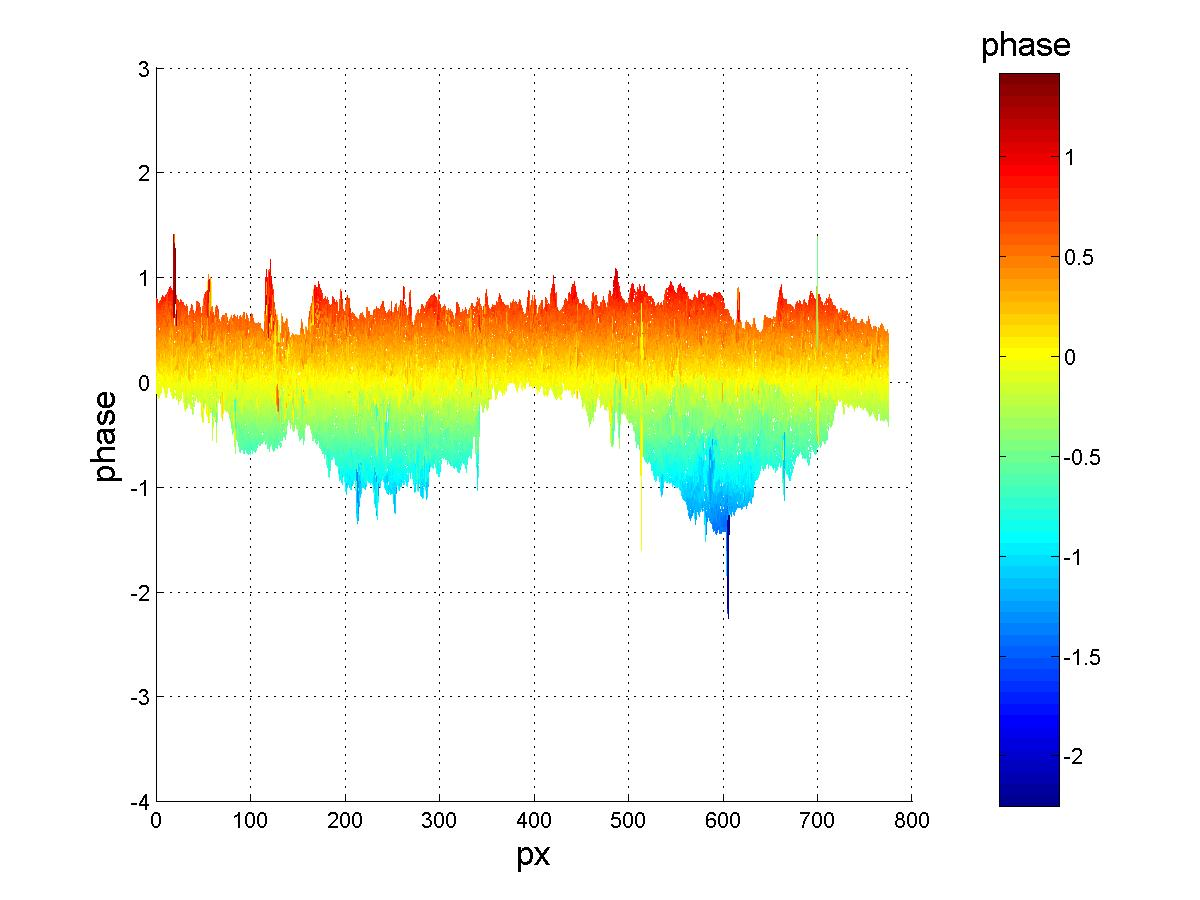
\includegraphics[width=0.5\textwidth]{figures/3DvBS_yz.jpg}}}	
	\subfigure[]{
		{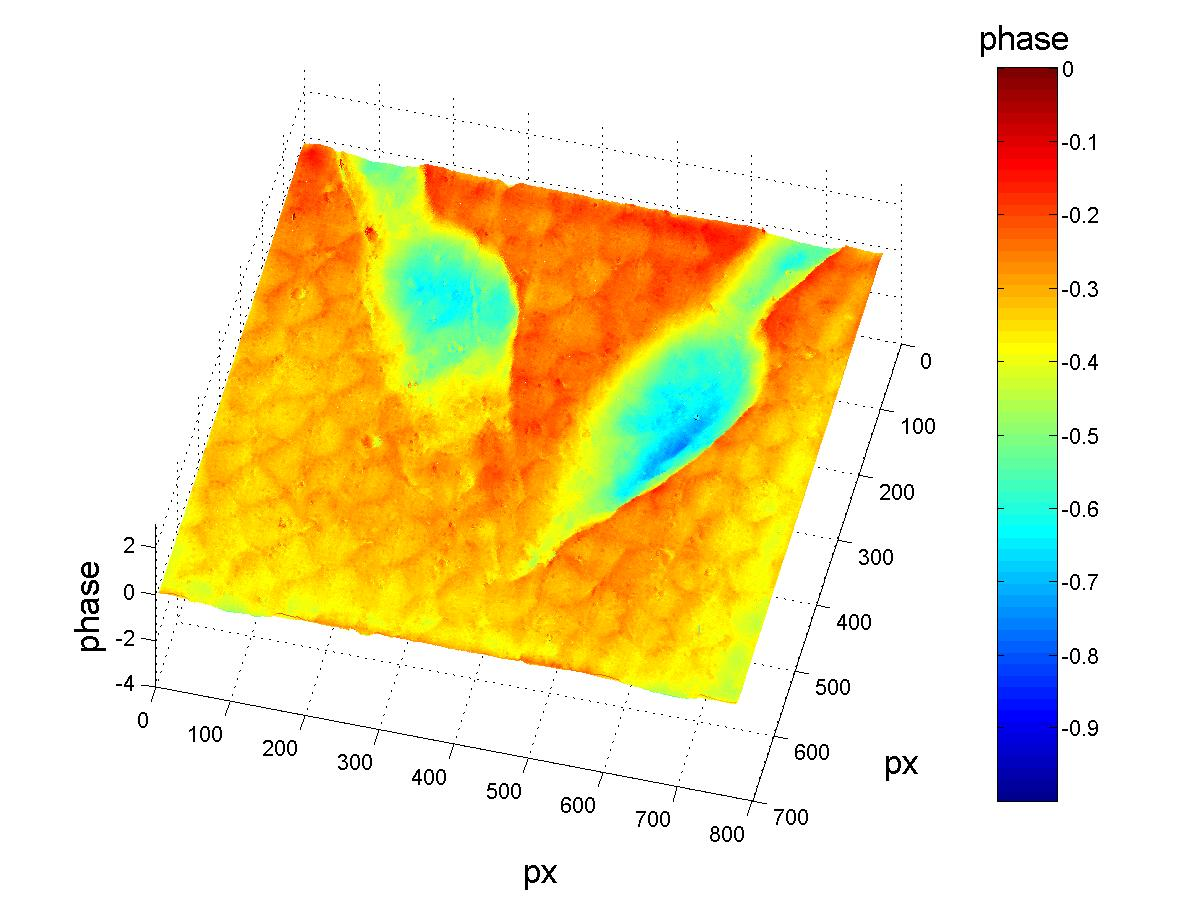
\includegraphics[width=0.5\textwidth]{figures/3Dvfiltered.jpg}}{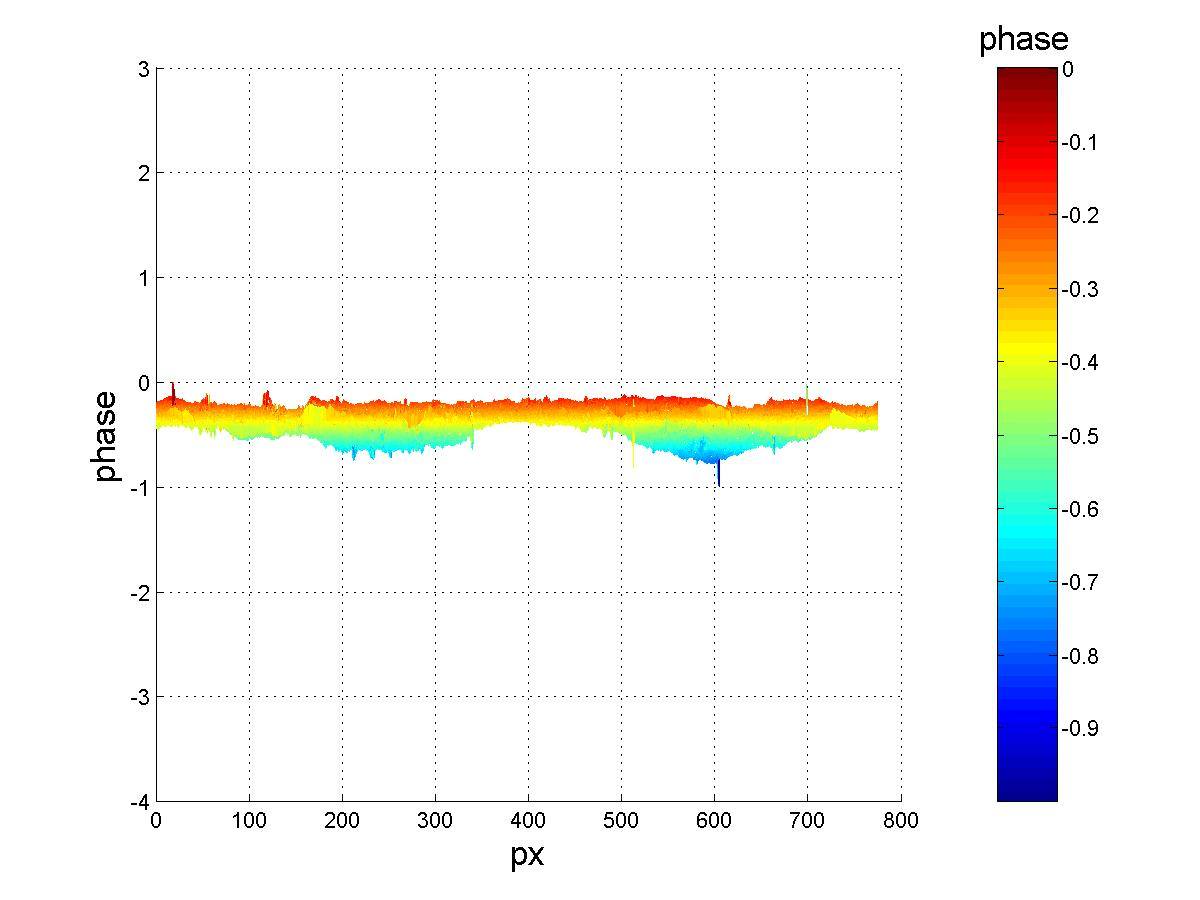
\includegraphics[width=0.5\textwidth]{figures/3Dvfiltered_yz.jpg}}}
	\caption[3D reconstruction of styrofoam with engraving]{3D (left) and yz-axis (right) view of Figure 5.2: (a) unprocessed (b) after removal of vignetting (c) after FFT-filtering.}
	\label{fig:3DV}
\end{figure}

For the pebbled wall (fig. \ref{fig:3Dstone}), the height of the pebbles and the gaps were measured with a caliper. Relative height of the pebbles were found to be ranging from 1 to 3 mm. The average depth of the gaps were measured to be 3 mm (ranging from 1 to 10 mm). As for the pyramid (fig. \ref{fig:3Dpyramid}), the exact heights of each step level (5mm) were accurately obtained. Peaks occuring at the edges are caused by the shadow of the edges when performing PSP.

\captionsetup[figure]{width=5in}
\begin{figure}[h!]
	\centering
	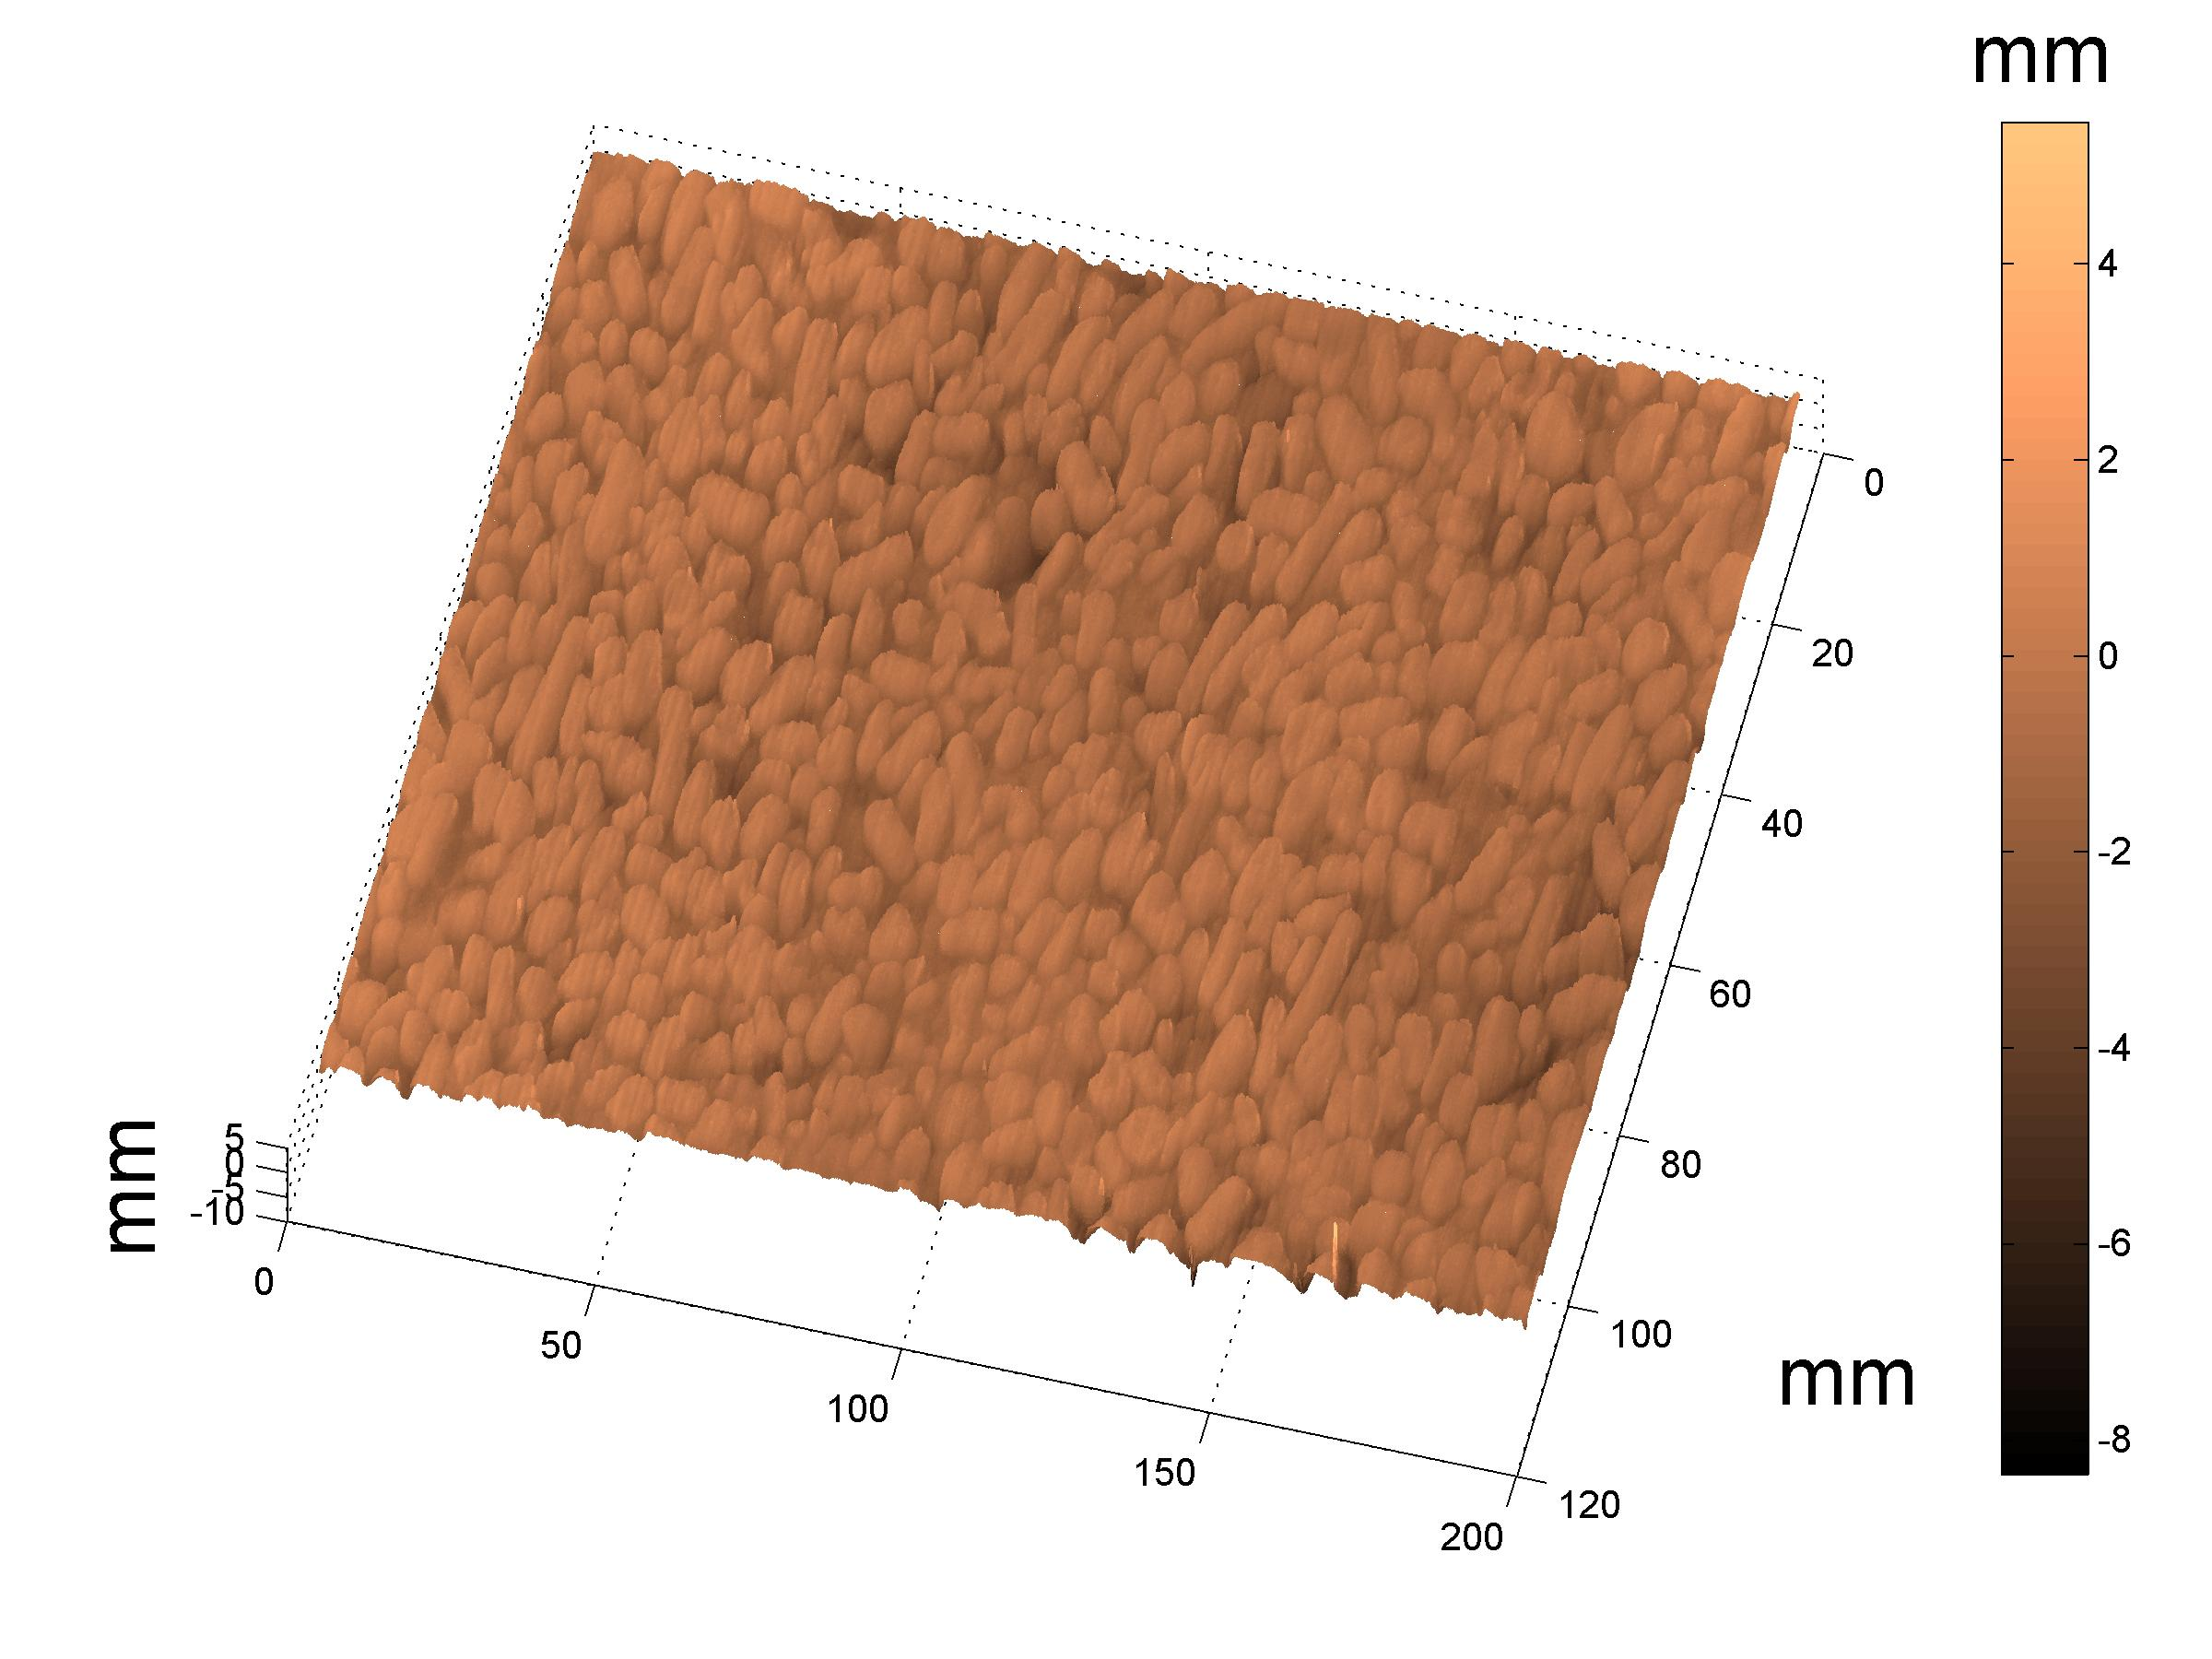
\includegraphics[width=0.6\textwidth]{figures/3Dpebble.jpg}
	\caption{3D view of the pebbled wall.}
	\label{fig:3Dstone}
\end{figure}


\captionsetup[figure]{width=5.2in}
\begin{figure}[h!]
	\centering
	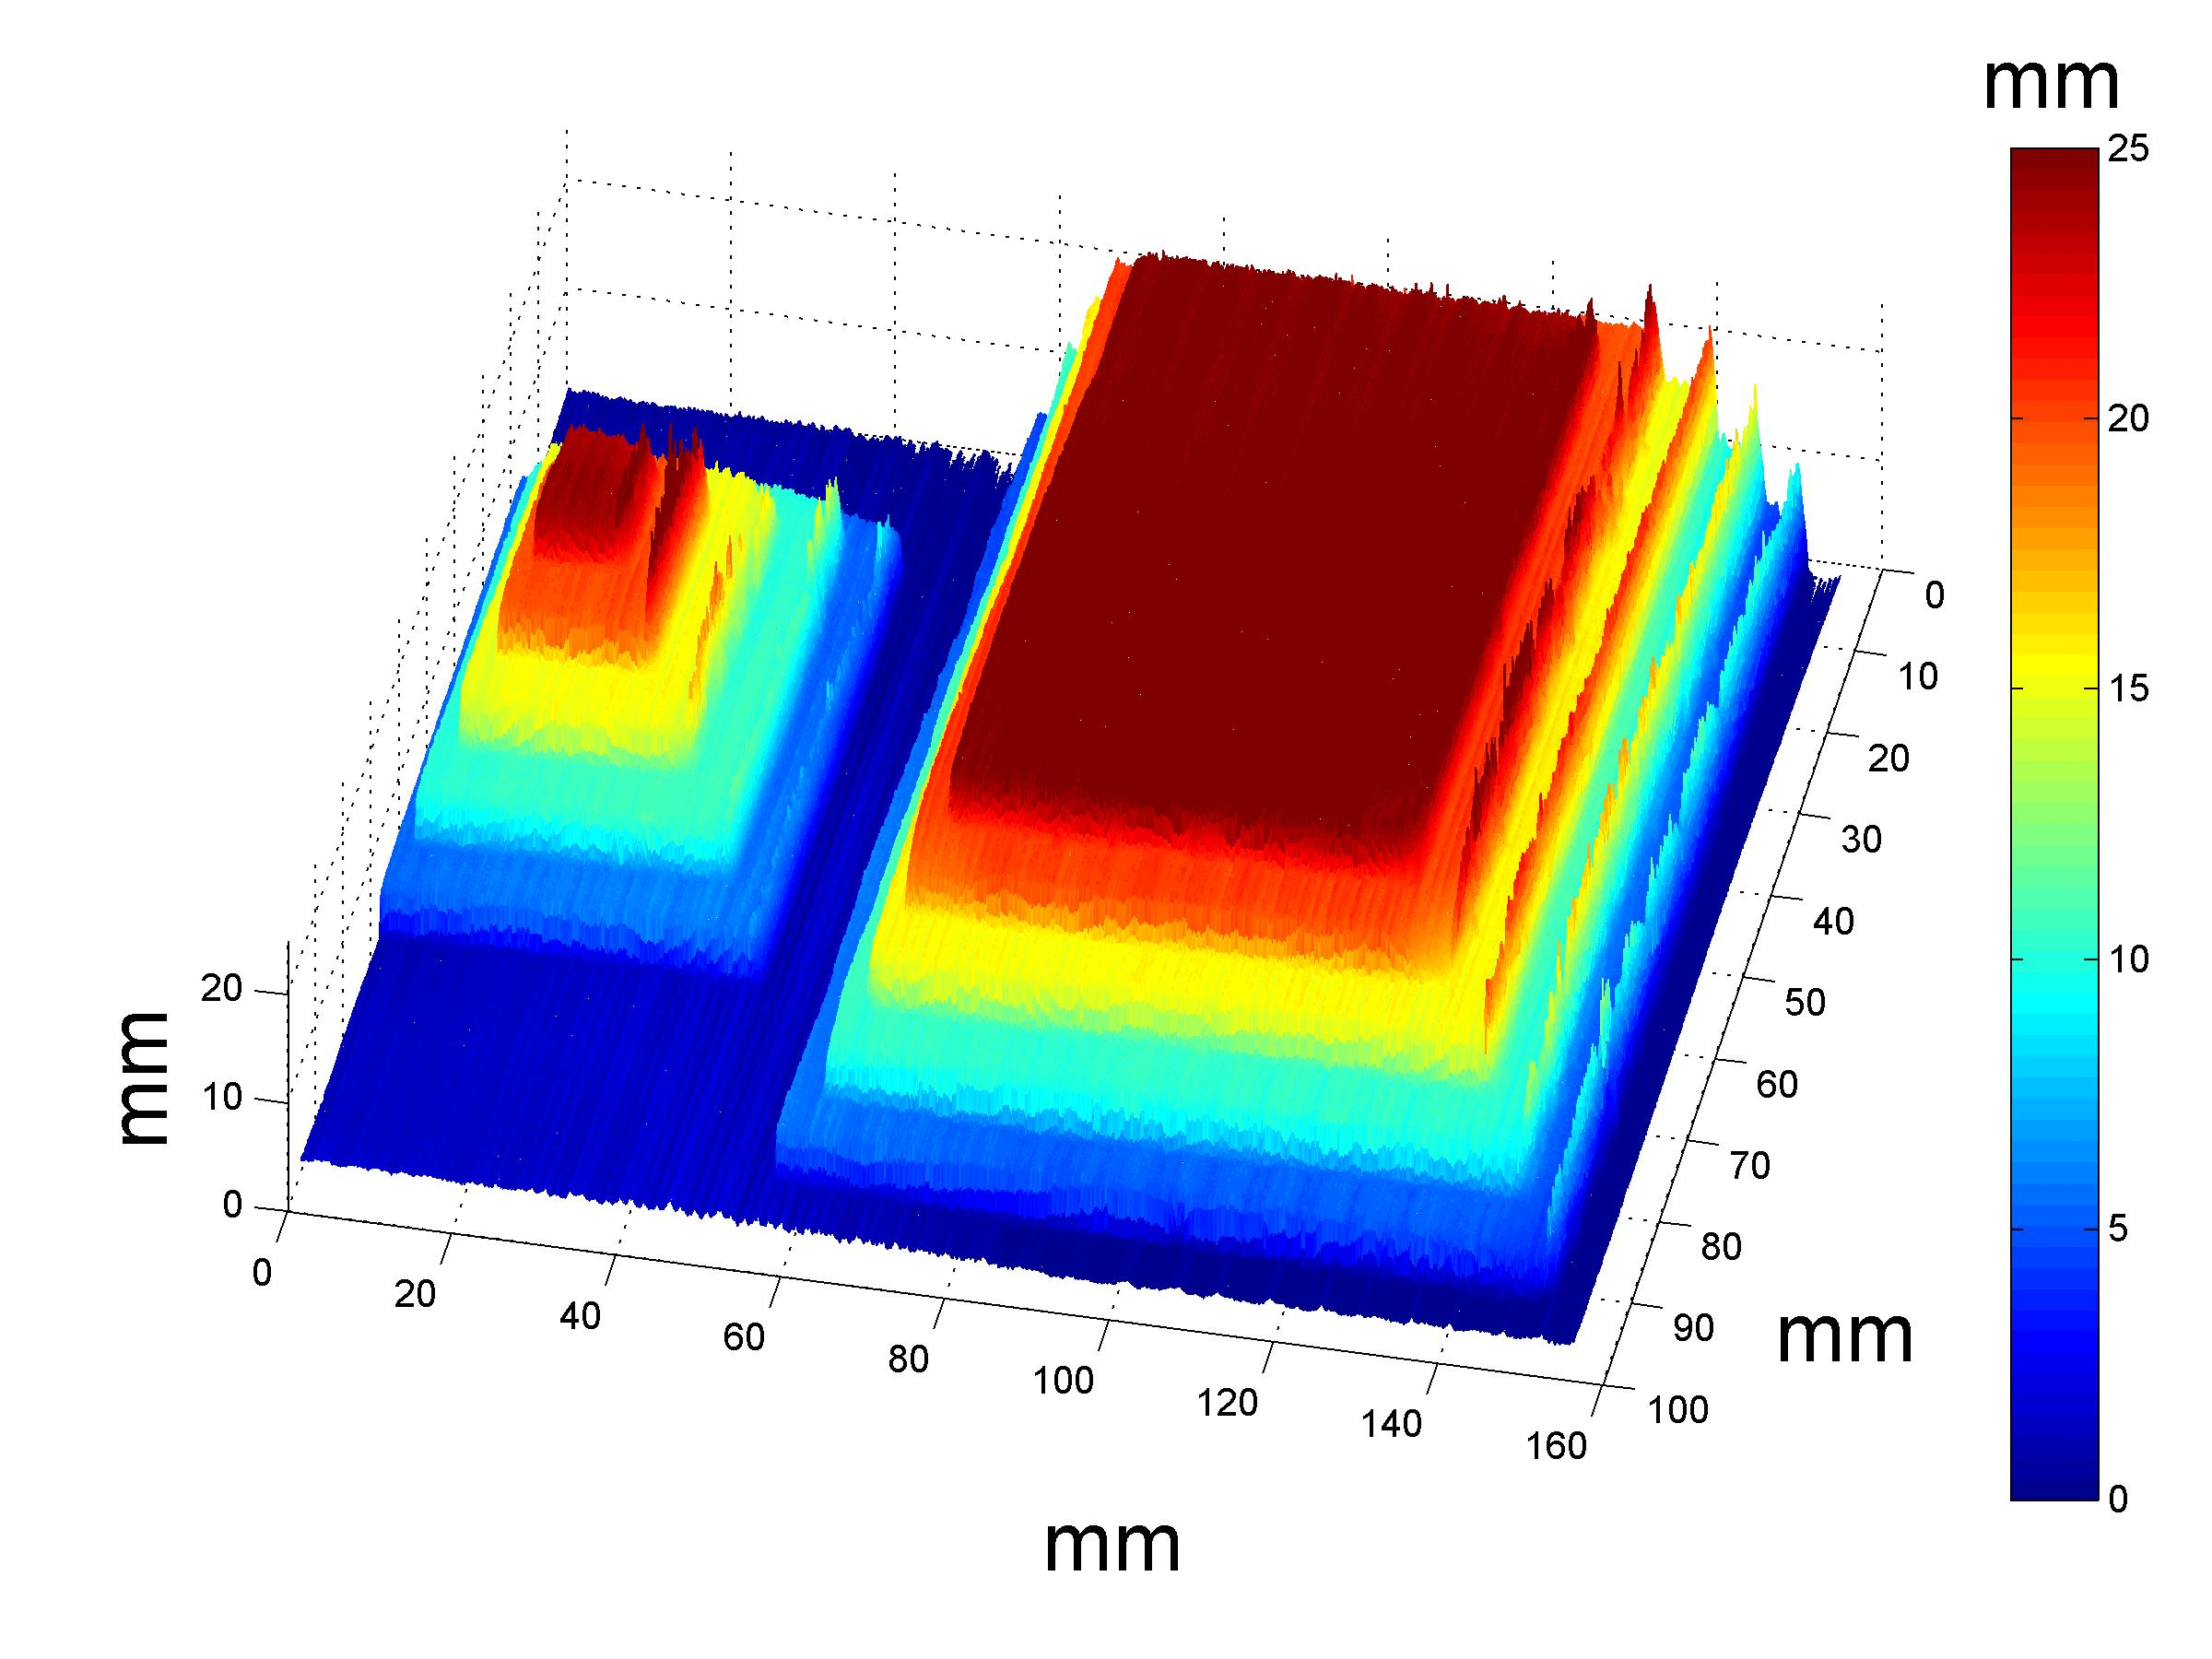
\includegraphics[width=0.55\textwidth]{figures/3Dpyramid.jpg}
	\caption[3D view of the step pyramid]{3D view of the step pyramid. Note that the height levels of 5 mm for each step was accurately obtained. The peaks occuring at the edges are caused by the shadows of the edges when performing PSP.}
	\label{fig:3Dpyramid}
\end{figure}

\section{3D Reconstruction of Scale Models of Angono Petroglyphs}

\subsection{Replica of Angono Petroglyphs}

Replica of some characters in the Angono were made by making use of the scanned stencils of the petroglyphs by Peralta \cite{Peralta1973}. A scale was provided in the scanned stencils and the actual measurements of the characters were measured using ImageJ\footnote{ImageJ is a free, open-source image processing software developed by the National Institutes of Health} software. Samples of the scanned stencils and their replica are shown in Figure \ref{fig:angono}. Note that the stencils are numbered - not in parentheses. Thus, we will refer to the petroglyphs based on these numbers: A-15, A-20, A-30, A-32, respectively, where A stands for Angono.

The replica were made since we were not allowed to visit the Angono petroglyphs heritage site due to its renovation (Dec. 2014 to date).  They are however approximately 1:1 scale models of the actual petroglyphs engraved in an acrylic-painted styrfoam to somehow mimic the color of the rocks were they are found.

\begin{figure}[h!]
	\centering
	\subfigure[A-15]{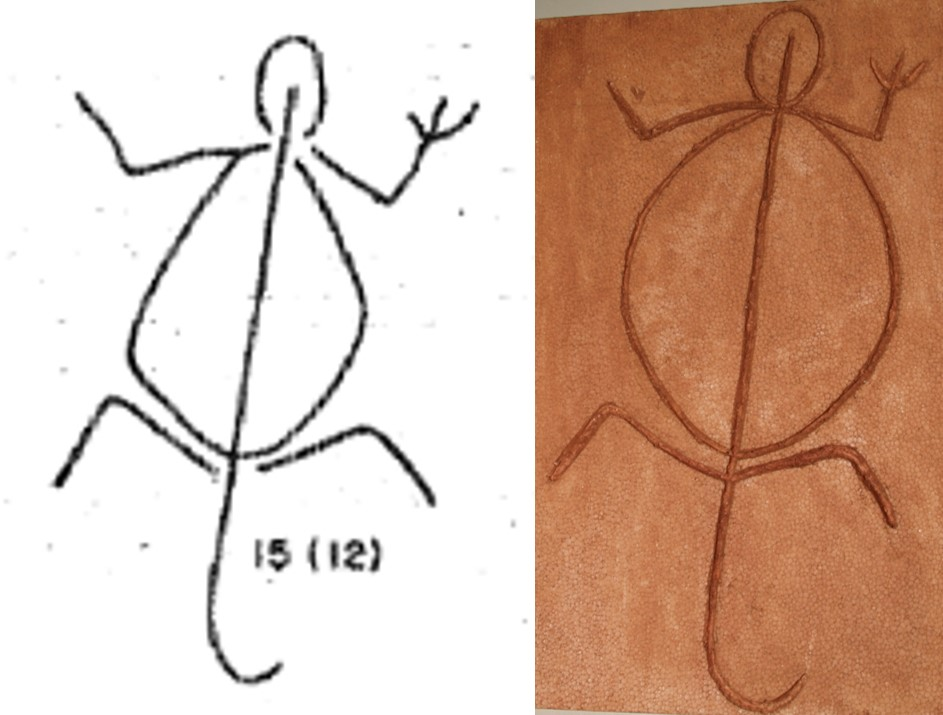
\includegraphics[width=0.45\textwidth]{figures/angono15.jpg}}
	\subfigure[A-20]{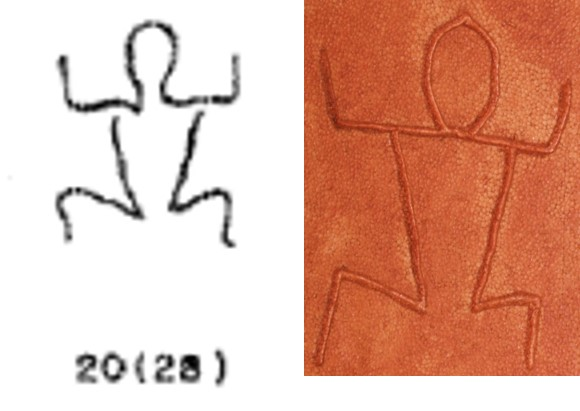
\includegraphics[width=0.45\textwidth]{figures/angono20.jpg}}
	\subfigure[A-30]{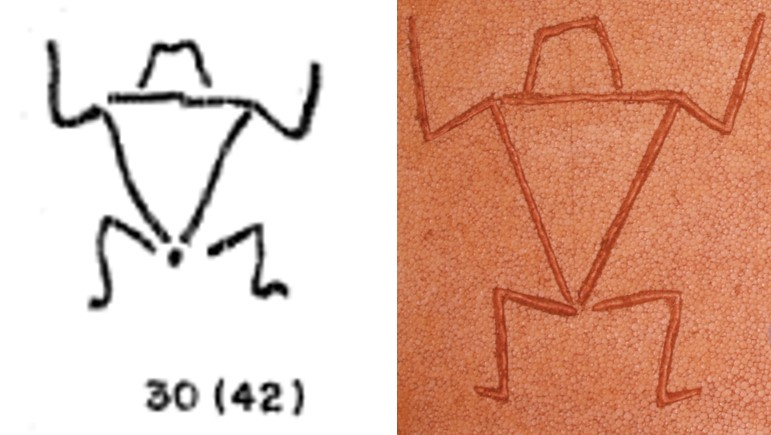
\includegraphics[width=0.45\textwidth]{figures/angono30.jpg}}
	\subfigure[A-30]{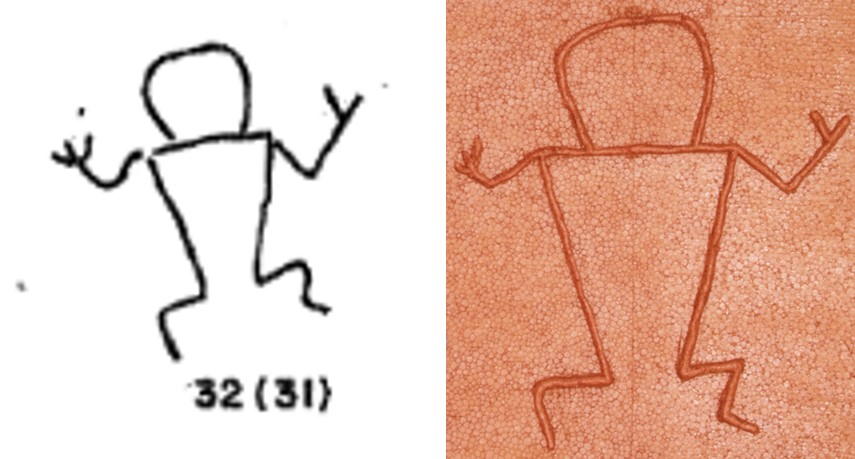
\includegraphics[width=0.45\textwidth]{figures/angono32.jpg}}	
	\caption[Stencils and replica of Angono petroglyphs]{Stencils (left) and replica (right) of some of the characters in the Angono petroglyhs.}
	\label{fig:angono}
\end{figure}


%\captionsetup[figure]{width=5in}
%\begin{figure}[h!]
%	\centering
%	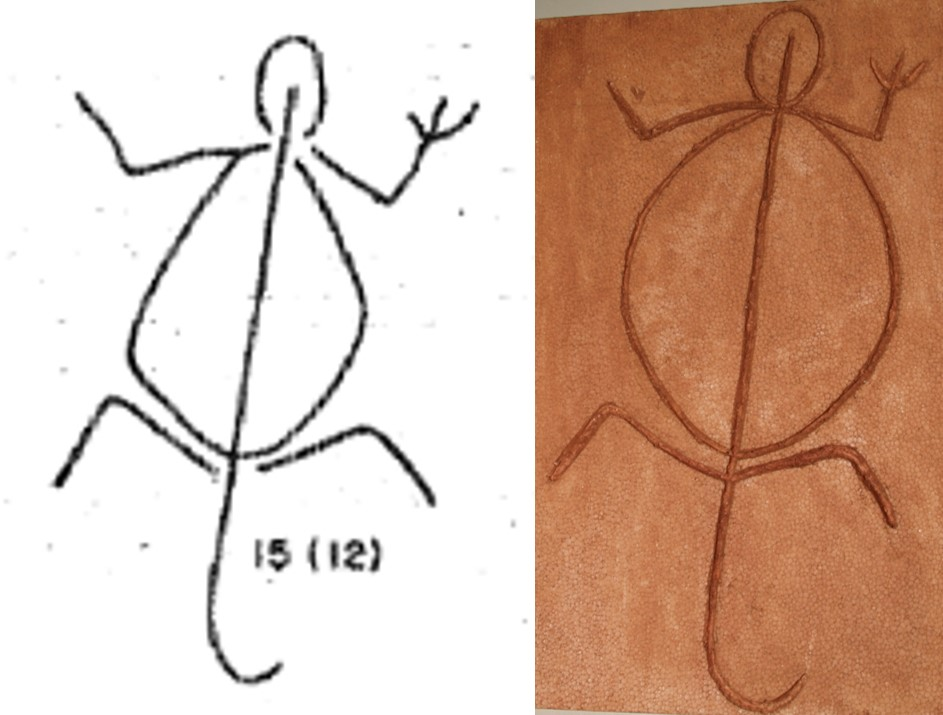
\includegraphics[width=0.45\textwidth]{figures/angono15.jpg}
%	\caption{A-15: A stencil and replica of one of the character in the Angono petroglyhs.}
%	\label{fig:angono15}
%\end{figure}
%
%\captionsetup[figure]{width=5in}
%\begin{figure}[h!]
%	\centering
%	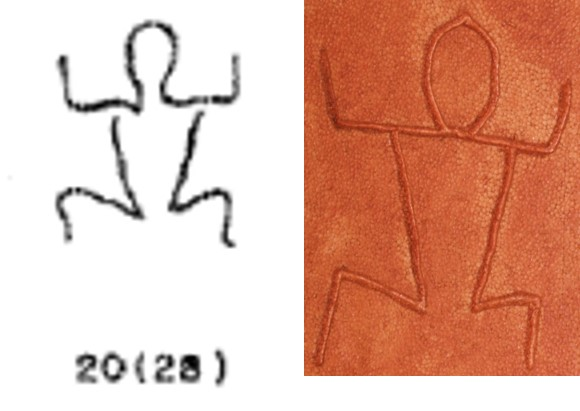
\includegraphics[width=0.4\textwidth]{figures/angono20.jpg}
%	\caption{A-20: A stencil (left) and replica (right) of one of the character in the Angono petroglyhs.}
%	\label{fig:angono20}
%\end{figure}
%
%\captionsetup[figure]{width=5in}
%\begin{figure}[h!]
%	\centering
%	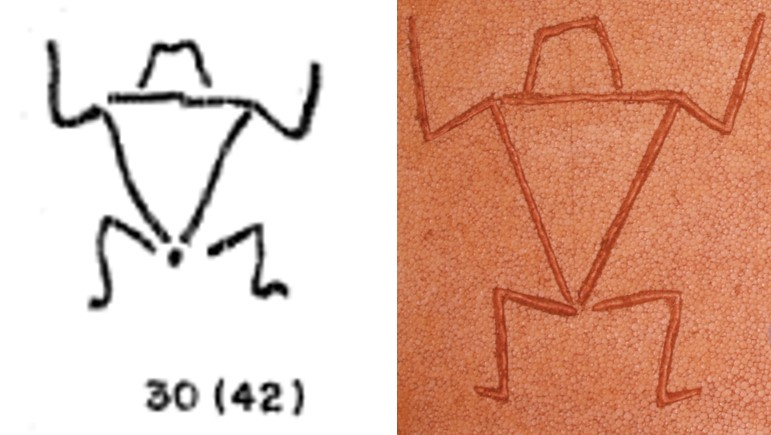
\includegraphics[width=0.4\textwidth]{figures/angono30.jpg}
%	\caption{A-30: A stencil and replica of one of the character in the Angono petroglyhs.}
%	\label{fig:angono30}
%\end{figure}

%\captionsetup[figure]{width=4in}
%\begin{figure}[h!]
%	\centering
%	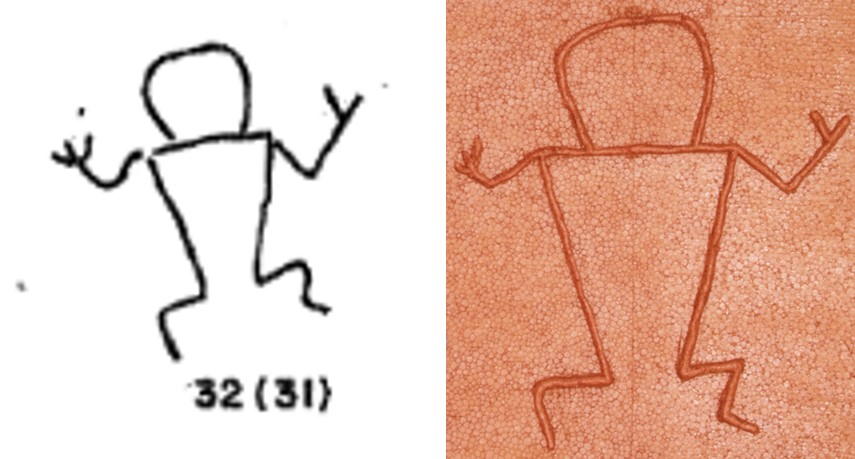
\includegraphics[width=0.4\textwidth]{figures/angono32.jpg}
%	\caption{A-32: A stencil and replica of one of the character in the Angono petroglyhs.}
%	\label{fig:angono32}
%\end{figure}

\subsection{3D Reconstruction with Depth Profile Analysis}

Sample 3D reconstructions of the Angono petroglyphs are shown in Figure \ref{fig:3Dangono}. Depth profile analysis along specific regions of A-20 was done by obtaining the height along the region after phase-to-height conversion. 

\begin{figure}[h!]
	\centering
	\subfigure[A-15]{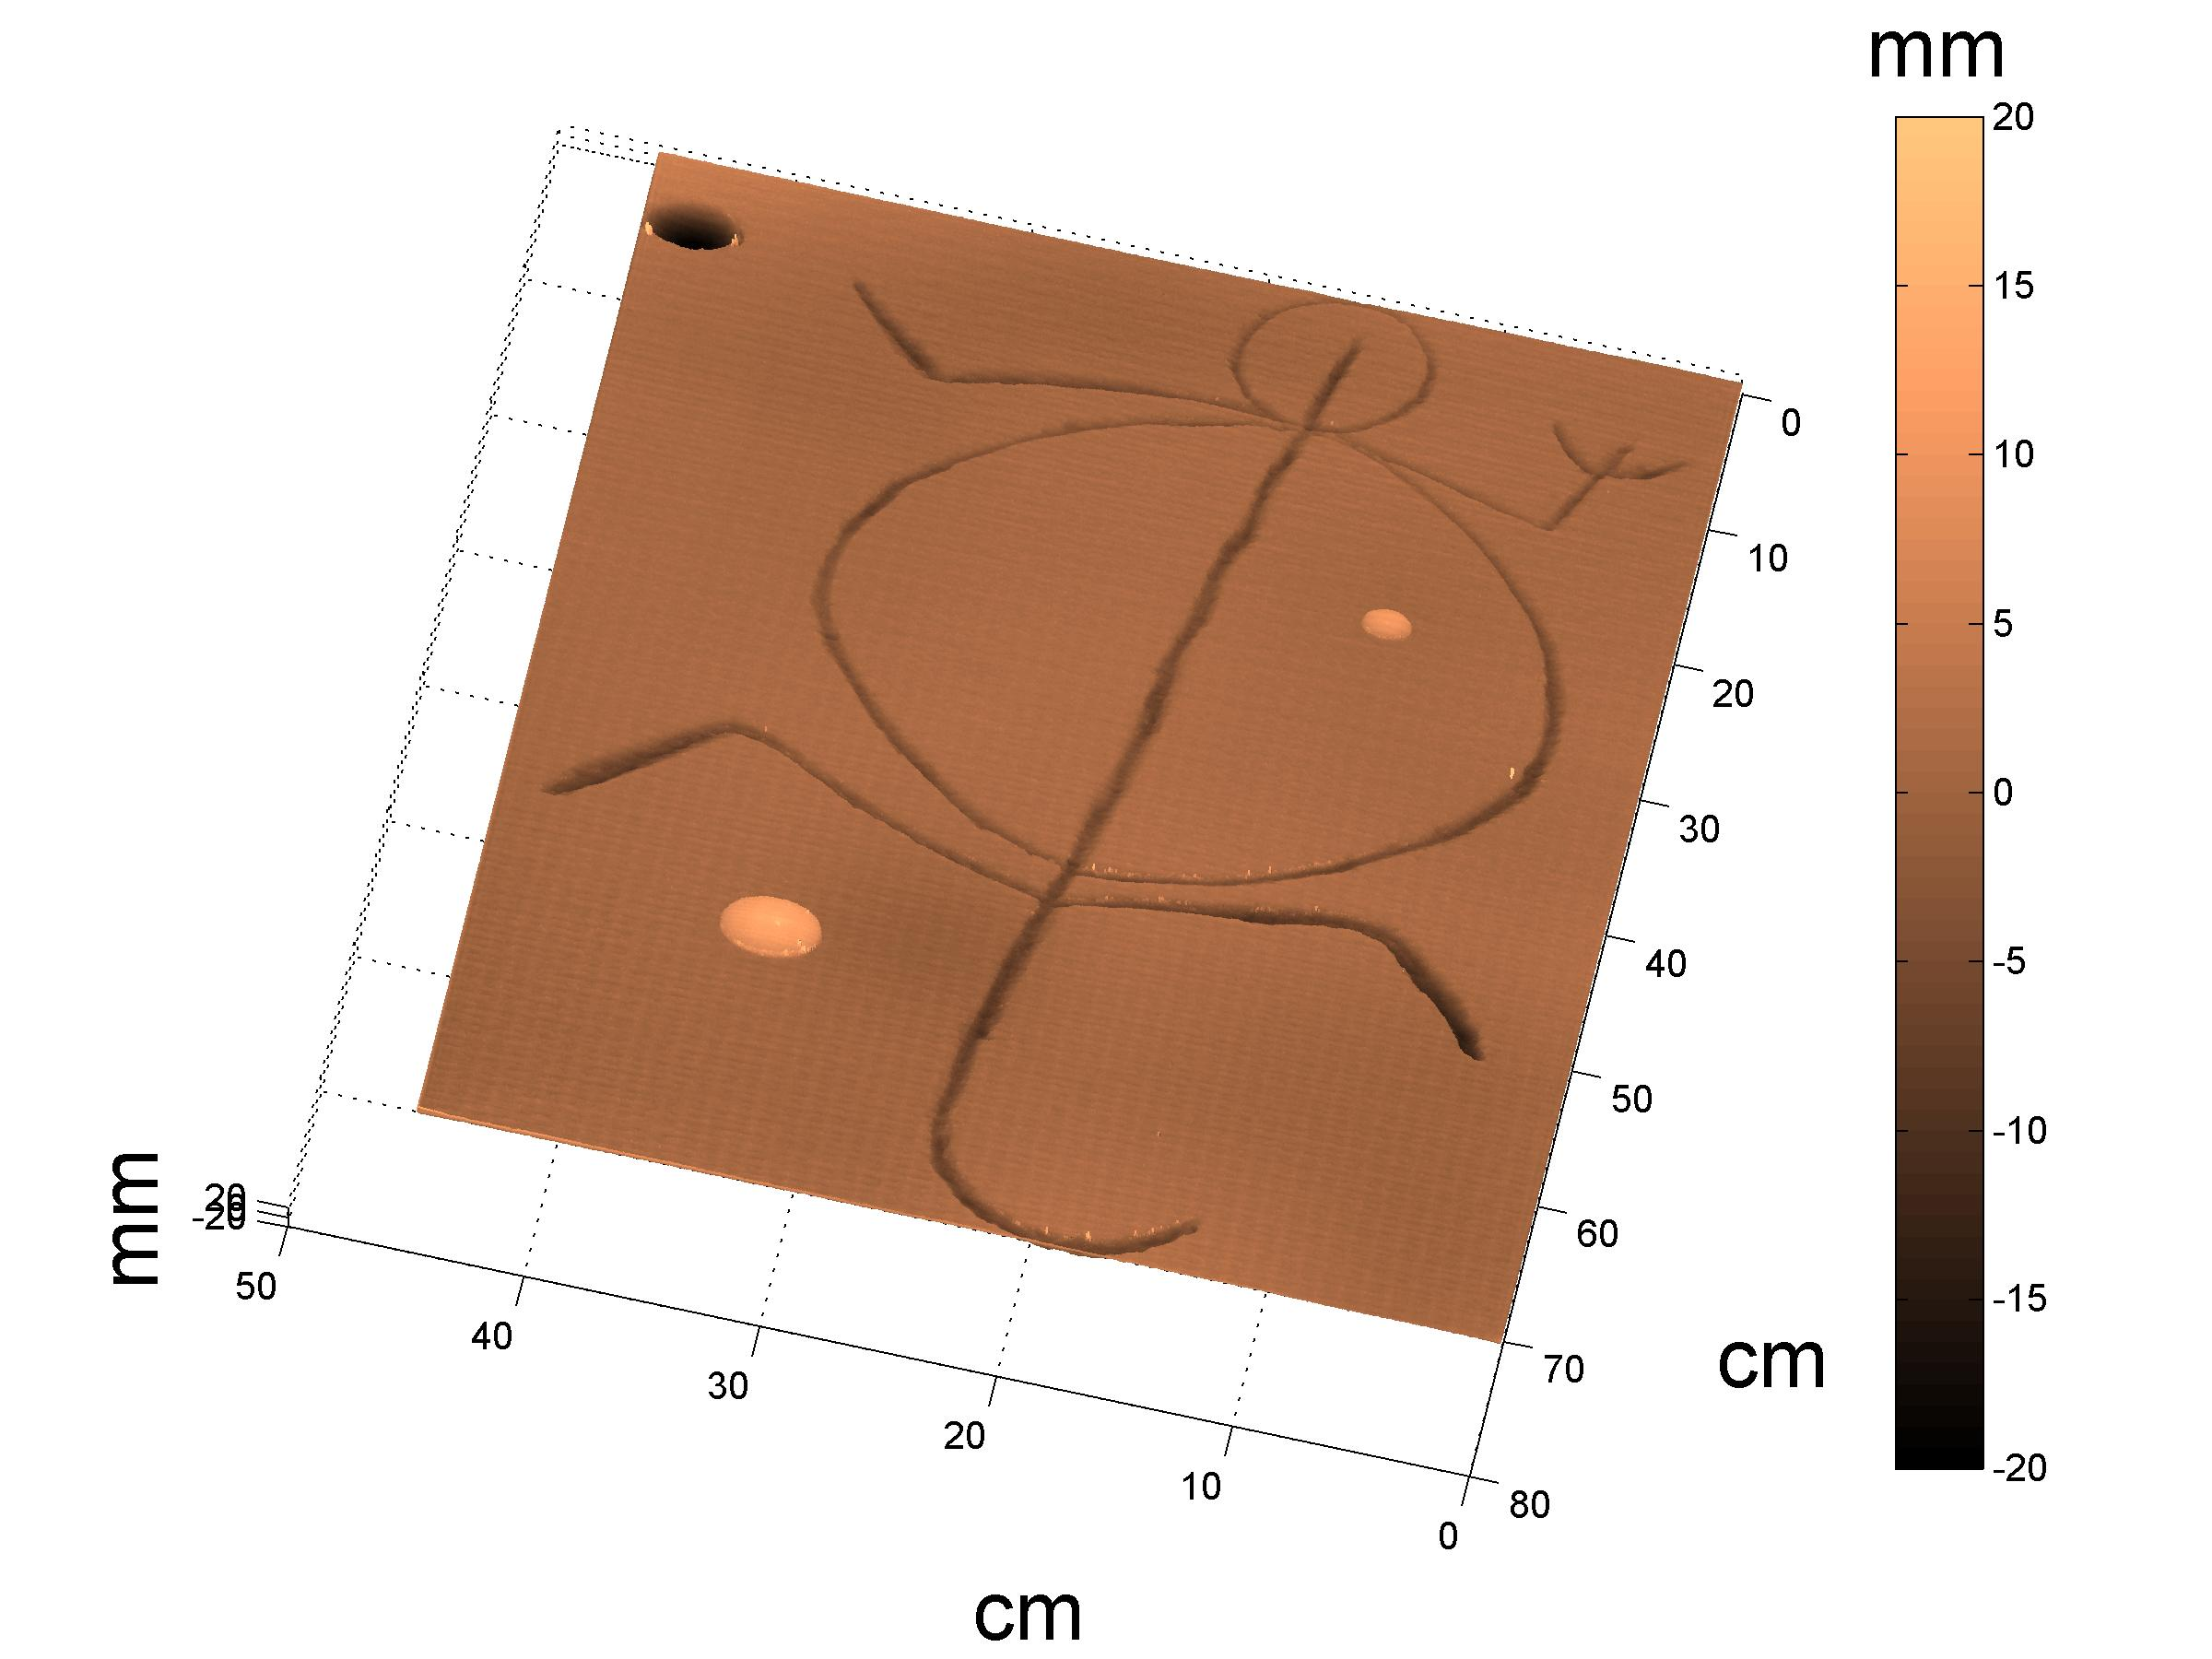
\includegraphics[width=0.48\textwidth]{figures/A15.jpg}}
	\subfigure[A-20]{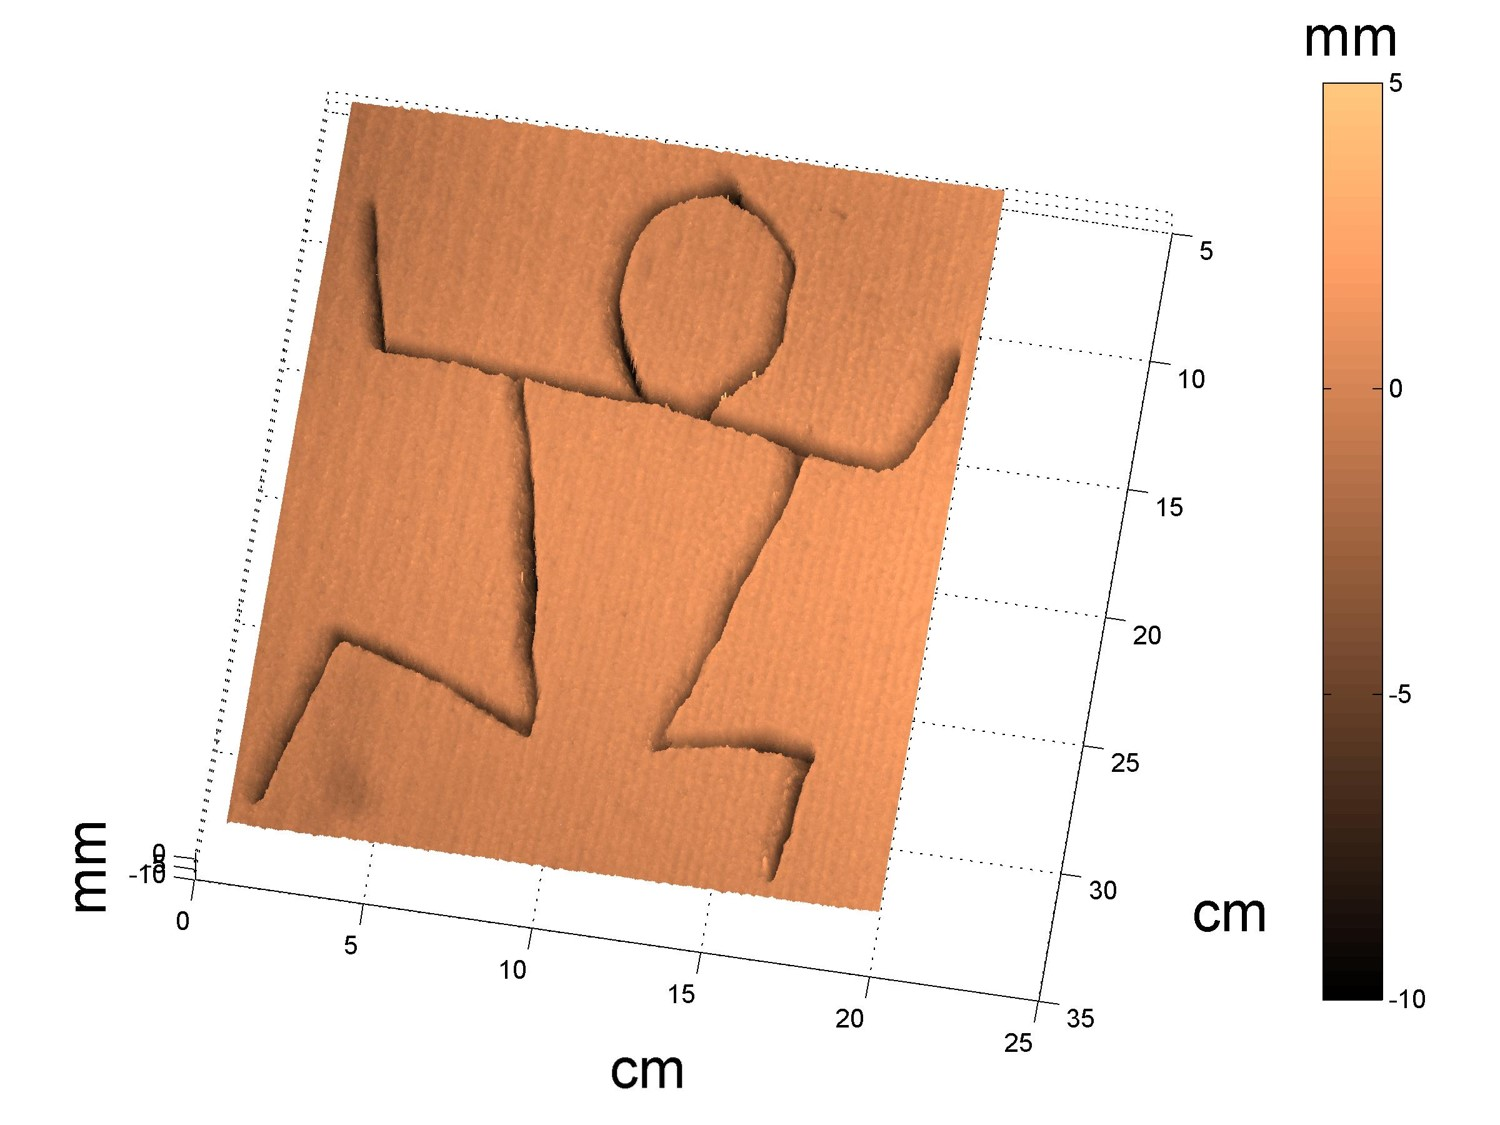
\includegraphics[width=0.48\textwidth]{figures/A20.jpg}}
	\subfigure[A-30]{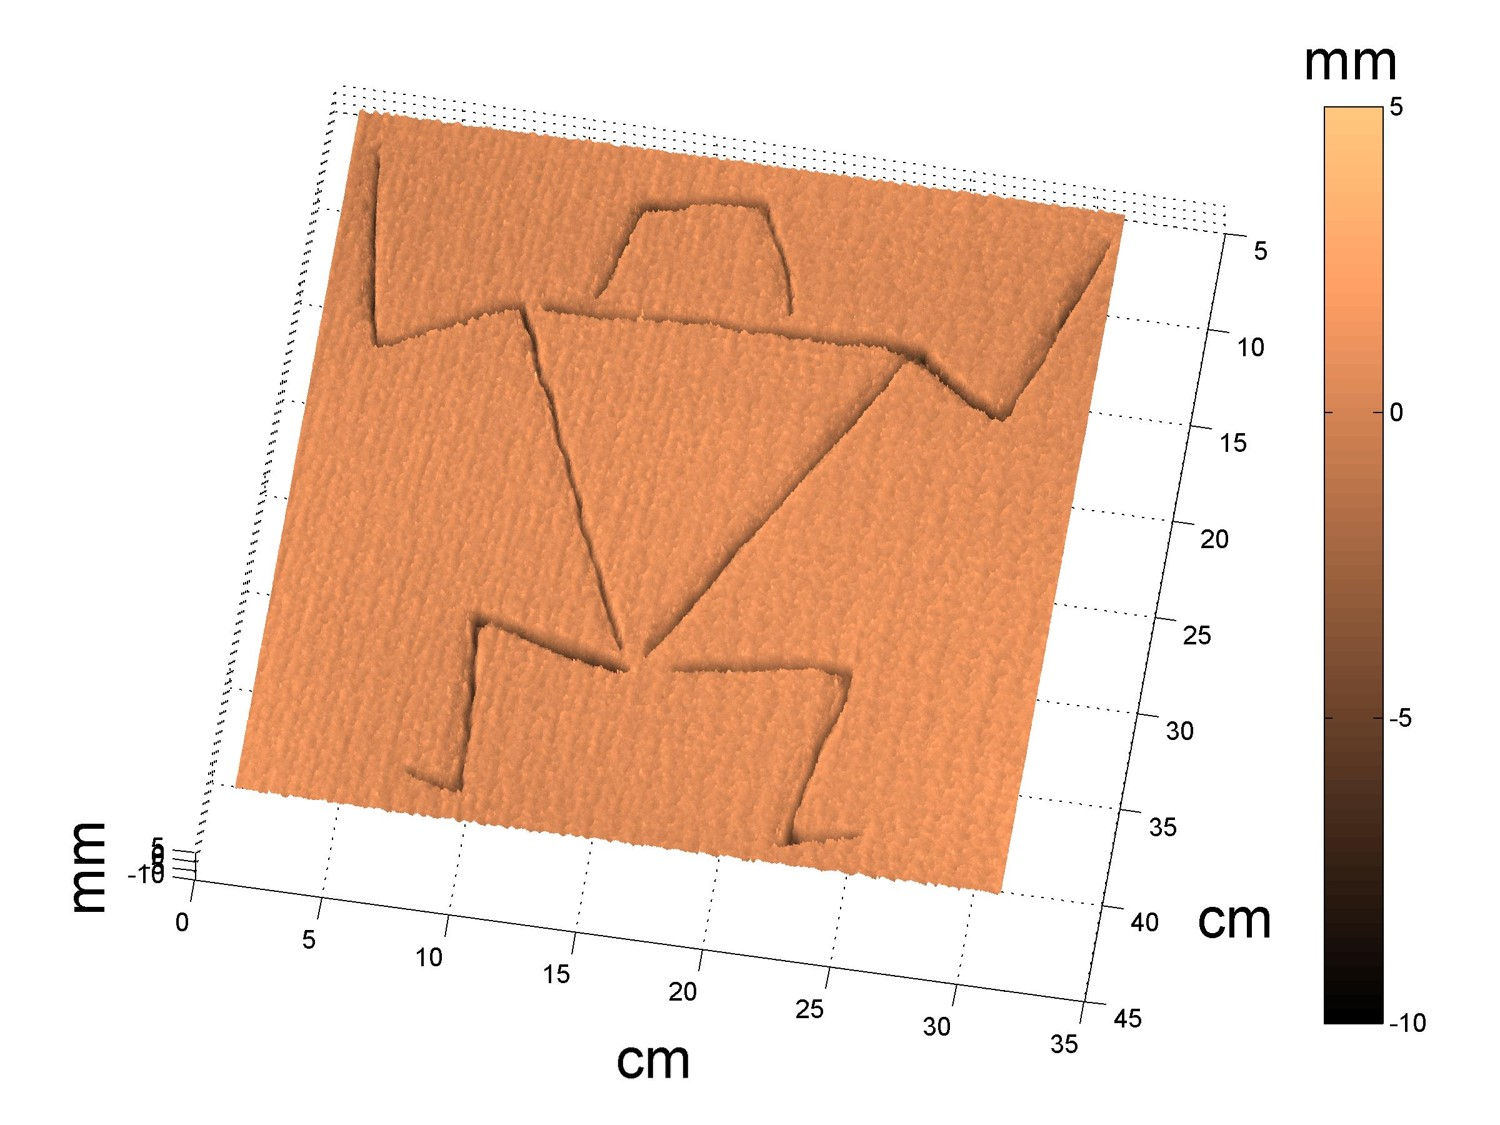
\includegraphics[width=0.48\textwidth]{figures/A30.jpg}}
	\subfigure[A-32]{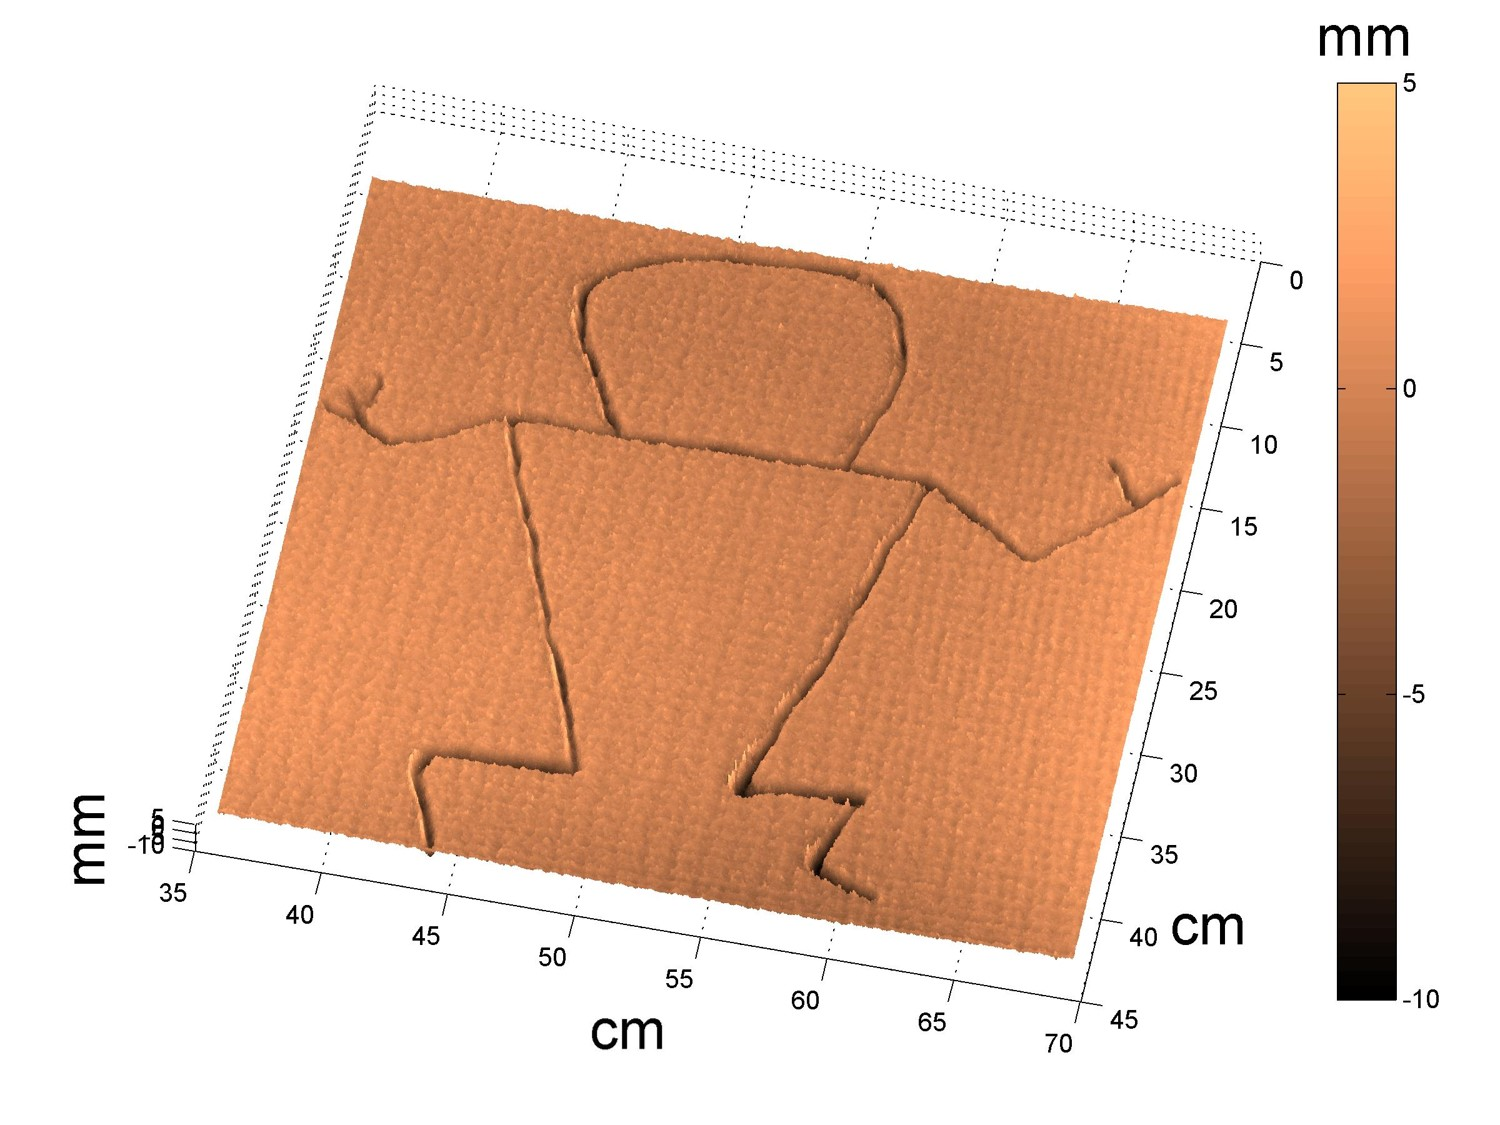
\includegraphics[width=0.48\textwidth]{figures/A32.jpg}}
	\caption[3D view of Angono petroglyphs replica]{3D mesh profiles of the Angono petroglpyhs replica. The white and black `dots' in A-15 are cut pingpong balls embedded on the styrofoam for height reference.}
	\label{fig:3Dangono}
\end{figure}

The sections chosen for analysis are along the `joints' wherein actual measurements were obtained using a caliper as shown in Figure \ref{fig:angono20}. Images of the scanned profile (along the regions) are shown in Figure \ref{fig:3Dangono20}.

As can be observed from the depth profiles, the lines are not that smooth. This can be attributed to the non-smooth surface of the styrofoam board itself as the characters were drawn. Also, they were drawn using a heated solder so the strokes are hardly controllable. 

Table \ref{tab:depth} shows the maximum depth values obtained from the caliper (actual) and PSP  measurements. We note that the caliper measurements has an uncertainty of $\pm$ 0.05 mm. A more accurate means of measuring the actual depth of the engravings may be employed to have better comparison of the actual and PSP measurements. Nonetheless, an average of 3.92\% error was obtained for the data of the depth measurements using PSP which verifies the accuracy of the data.

\captionsetup[figure]{width=5in}
\begin{figure}[h!]
	\centering
	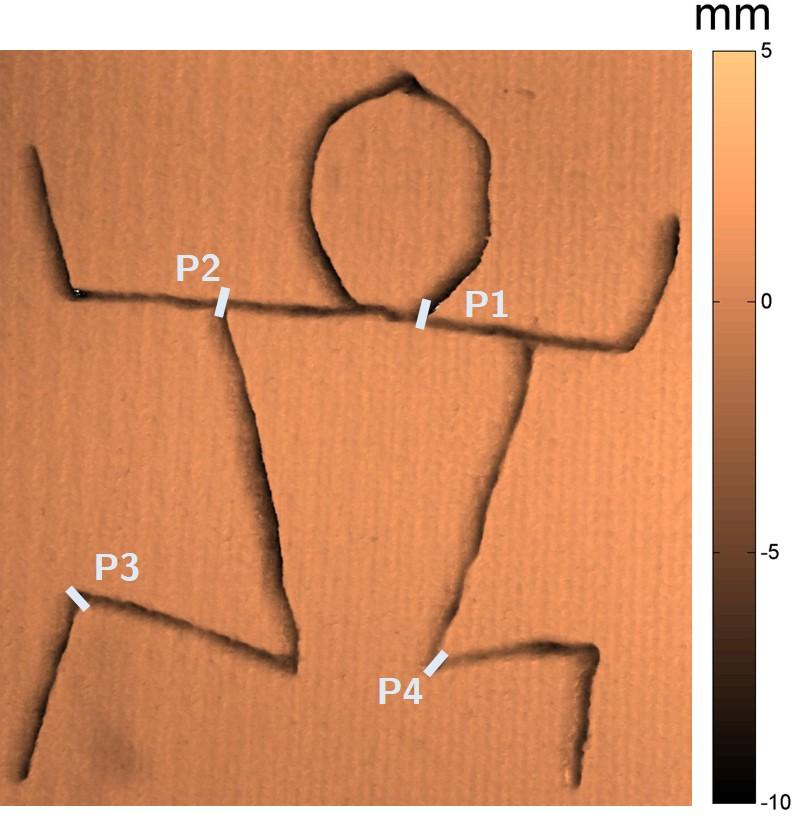
\includegraphics[width=0.45\textwidth]{figures/A20flat.jpg}
	\caption[Height map of sample Angono replica]{A-20: Highlighted regions are for depth profile analysis.}
	\label{fig:angono20}
\end{figure}

\begin{figure}[h!]
	\centering
	\subfigure[P1]{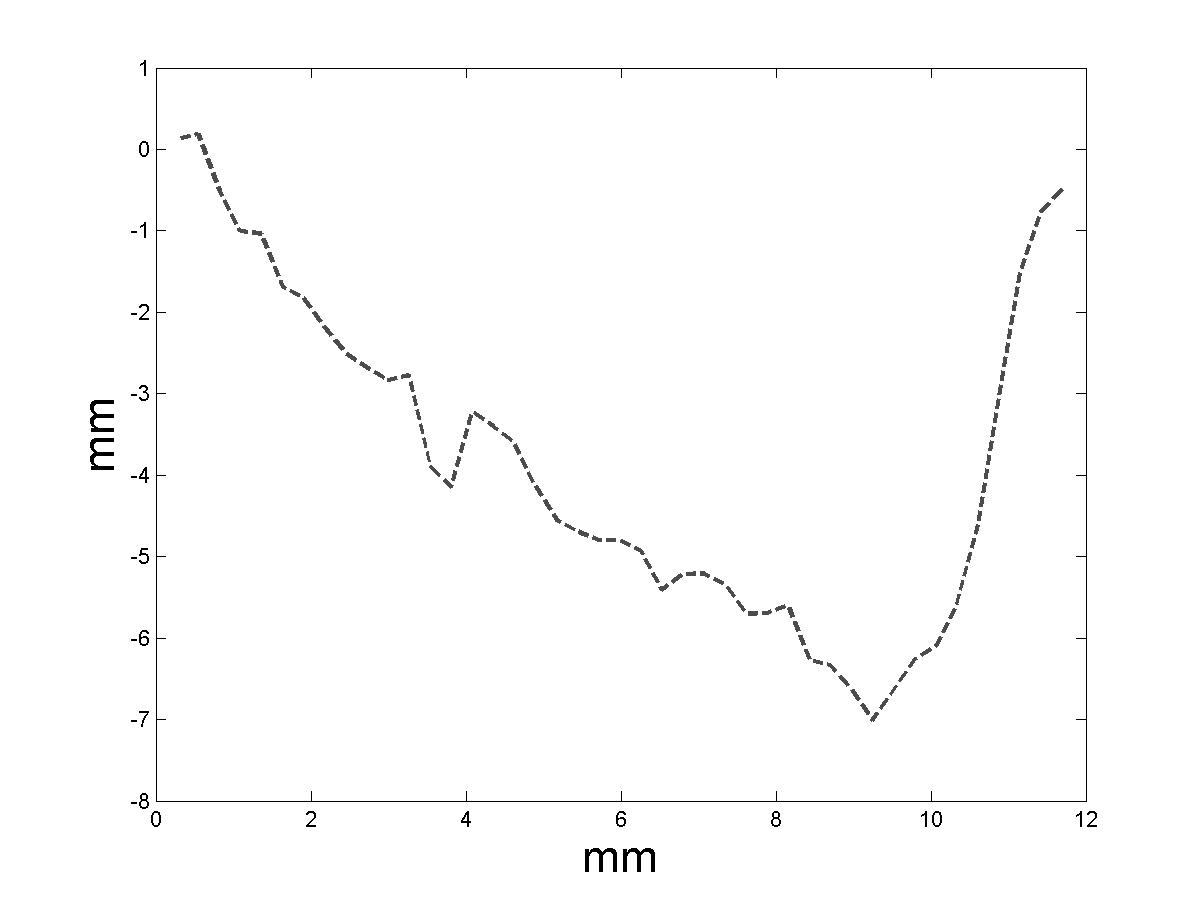
\includegraphics[width=0.45\textwidth]{figures/A20p1.jpg}}
	\subfigure[P2]{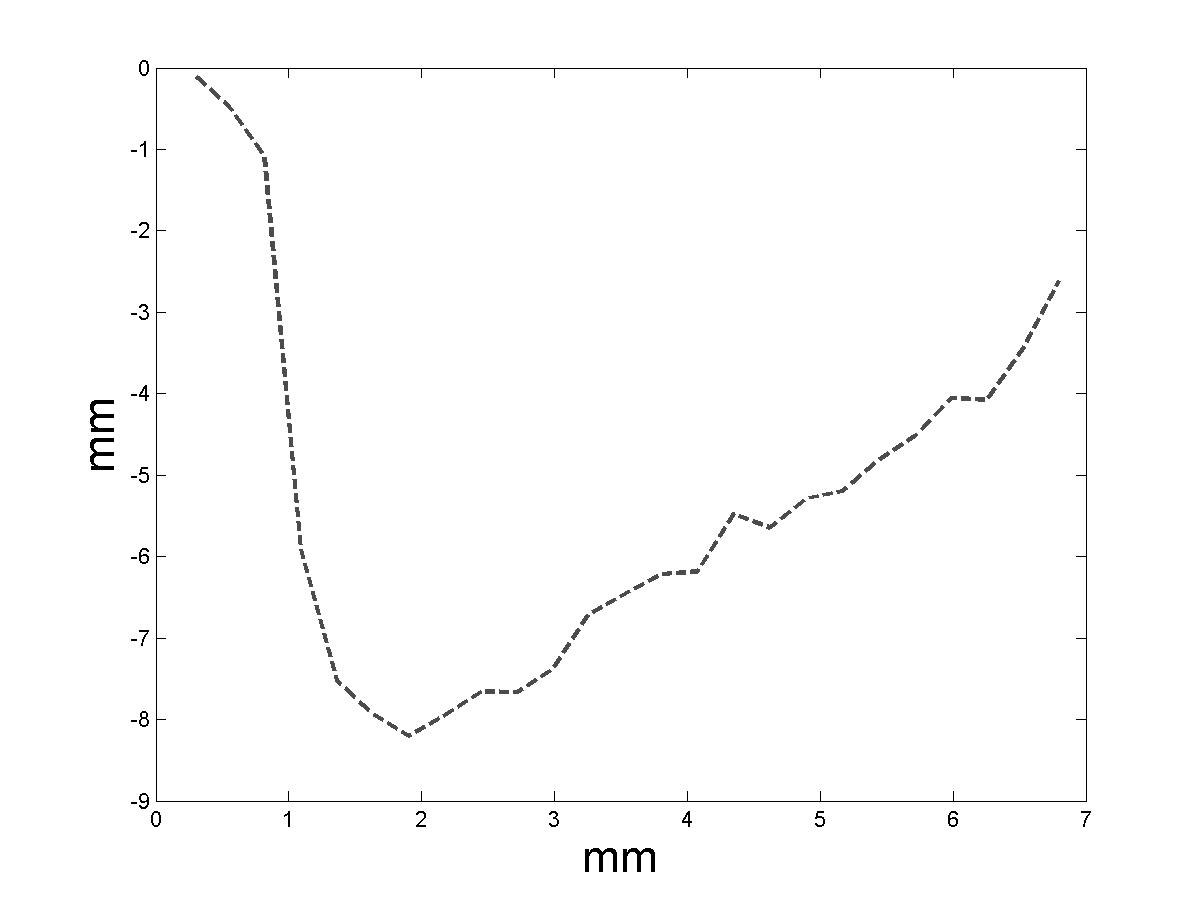
\includegraphics[width=0.45\textwidth]{figures/A20p2.jpg}}
	\subfigure[P3]{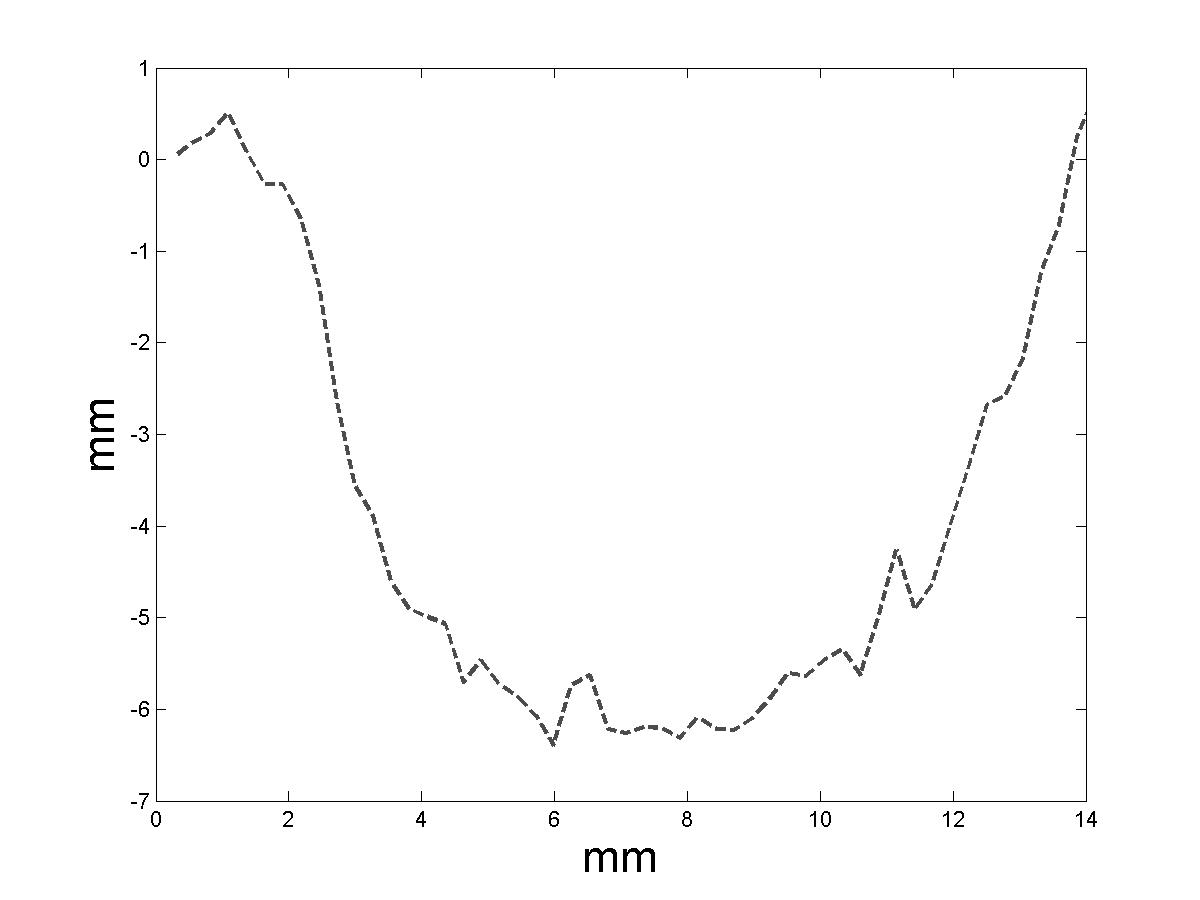
\includegraphics[width=0.45\textwidth]{figures/A20p3.jpg}}
	\subfigure[P4]{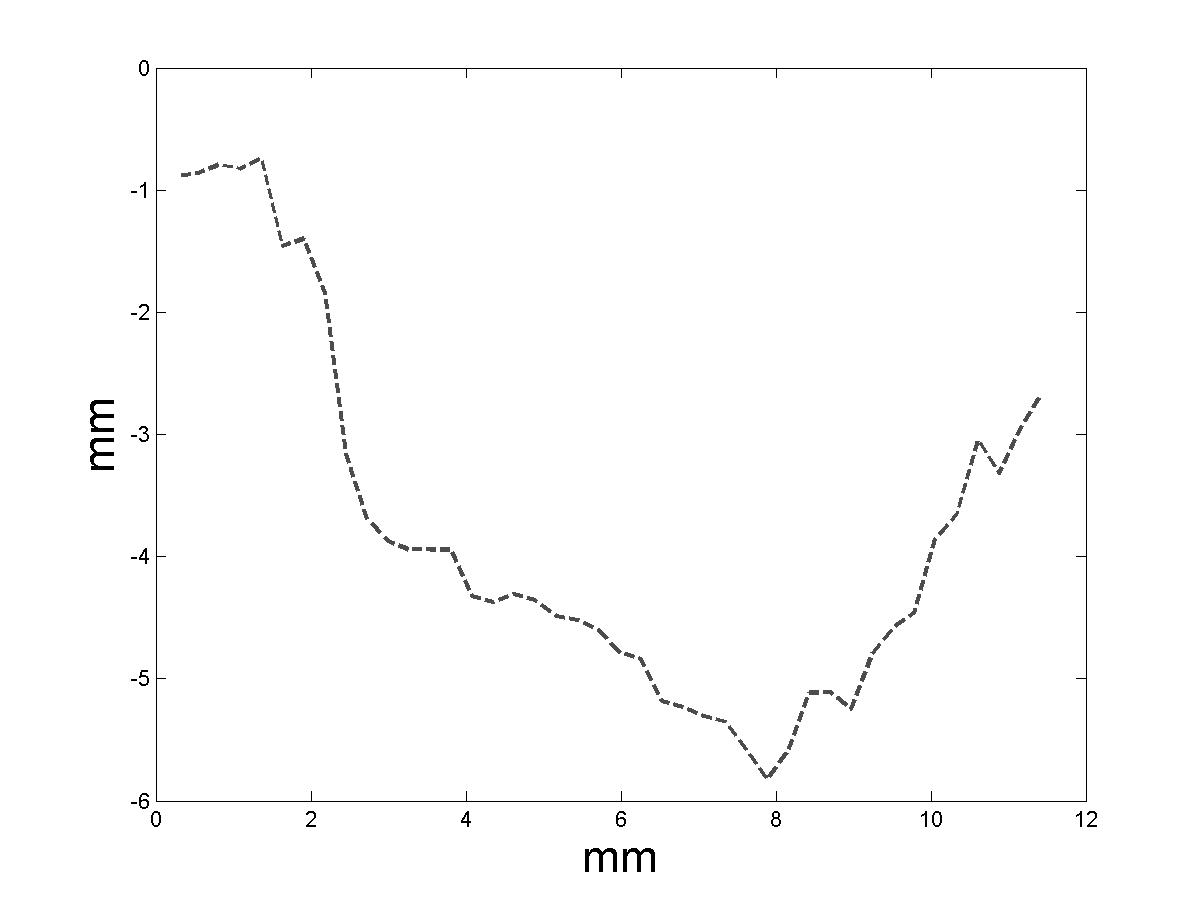
\includegraphics[width=0.45\textwidth]{figures/A20p4.jpg}}
	\caption[Depth profiles of sample Angono replica]{Sample depth profile analysis along the highlighted portions in A-20.}
	\label{fig:3Dangono20}
\end{figure}

\begin{table}[htbp]
	\centering
	\caption[Caliper and PSP obtained depth comparison of Angono petroglyph replica]{Caliper and PSP obtained depth comparison of A-20.}
	\begin{tabular}{rrrrr}
		\toprule
		&       & \multicolumn{3}{c}{Maximum Depth (mm)} \\
		\midrule
		&       & \multicolumn{1}{c}{Using Caliper ($\pm$ 0.05 mm)} & \multicolumn{1}{c}{PSP} & \multicolumn{1}{c}{\% error} \\
%		A-15 & P1 &       &       &  \\
%		& P2 &       &       &  \\
%		& P3 &       &       &  \\
%		& P4 &       &       &  \\
		A-20 & P1 & \multicolumn{1}{c}{6.80} & \multicolumn{1}{c}{7.10} & \multicolumn{1}{c}{4.4} \\
		& P2 & \multicolumn{1}{c}{8.10} & \multicolumn{1}{c}{8.20} & \multicolumn{1}{c}{1.3} \\
		& P3 & \multicolumn{1}{c}{6.20} & \multicolumn{1}{c}{6.40} & \multicolumn{1}{c}{3.2} \\
		& P4 & \multicolumn{1}{c}{5.45} & \multicolumn{1}{c}{5.82} & \multicolumn{1}{c}{6.9} \\
		\hline
		Average & &  &  & \multicolumn{1}{c}{3.92} \\
%		A-30 & P1 &       &       &  \\
%		& P2 &       &       &  \\
%		& P3 &       &       &  \\
%		& P4 &       &       &  \\
%		A-32 & P1 &       &       &  \\
%		& P2 &       &       &  \\
%		& P3 &       &       &  \\
%		& P4 &       &       &  \\
		\bottomrule
	\end{tabular}%
	\label{tab:depth}%
\end{table}%

